
\section{Das Android Betriebssystem}
	Das Unternehmen Android wurde 2003 von Andy Rubin gegr"undet und wurde 2005 von Google aufgekauft. Seitdem k"ummert sich Google und das Android Open Source Project (AOSP) um die Weiterentwicklung des Systems. Aktuell ist Android, mit 55.6\% Marktanteil\footnote{Kantar Worldpanel: Smartphone OS sales market share, http://www.kantarworldpanel.com/global/smartphone-os-market-share/, 17.5.2015}, das vorherrschende Betriebssystem f"ur mobile Endger"ate in den USA.
	\\\\
	Basis für das Betriebssystem ist ein modifizierter Linux-Kernel und eine Java Virtual Machine (JVM). Bis einschliesslich Version 4.4 wurde hierf"ur die Dalivk Runtime und für alle neueren Versionen die Android Runtime (ART) verwendet. Jede App l"auft in einer eigenen Instanz der entsprechenden Runtime und damit in einer Sandbox.\newline
	Oberhalb der JVM sind die meisten Komponenten in Java implementiert. 
	
	\begin{figure}[h]
		\centering
		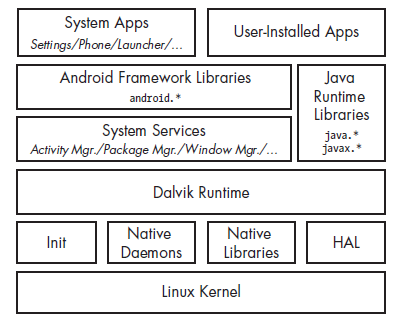
\includegraphics[width=0.7\linewidth]{android_pages/graphics/architektur_android_.png}
		\caption{Die Architektur von Android ASI-P-2}
		\label{fig:architektur_android}
	\end{figure}